\subsection{Results}
The robot sweeps all reachable floor space.
The total traveled path length is 80541.2 m, corresponding to a travel time of 16 hours and 7 minutes.

Figure \ref{floor_sweeping_results} shows part of the offline generated map vs. the traveled path in the same part of the map.

The offline planning part of the code takes about 30 seconds to execute,
while the robot movement code runs for approximately 6 minutes.

\begin{figure}[ht]
\centering
  \begin{subfigure}[t]{0.3\textwidth}
    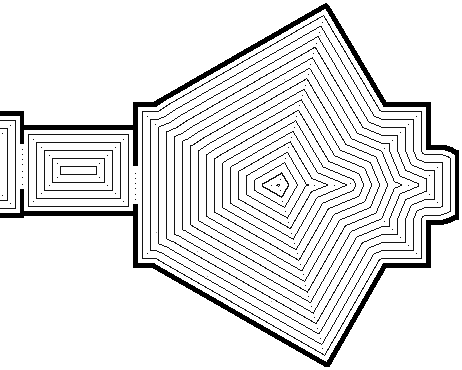
\includegraphics[width = \textwidth]{graphics/floor_sweep_plan}
    \caption{Part of the offline generated map for floor sweeping. The coordinates in \(S_{F}\) are marked.}
    \label{floor_sweep_plan}
  \end{subfigure}
  \begin{subfigure}[t]{0.3\textwidth}
    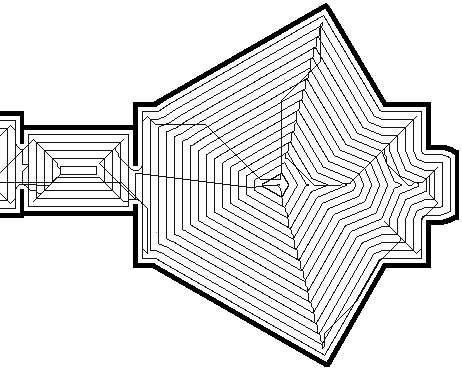
\includegraphics[width = \textwidth]{graphics/floor_sweep_robot}
    \caption{Part of the traveled path in floor sweeping. The coordinates visited are marked.}
    \label{floor_sweep_robot}
  \end{subfigure}
\caption{Floor sweeping planned vs. traveled}
\label{floor_sweeping_results}
\end{figure}